\section{Formation time}

\begin{slide}[toc=LP effect]{Landau Pomeranchuk effect}
  
    \rput(0.75\slidewidth, 0.17\slideheight)
    {
    \scalebox{0.6}
    {
    \begin{pspicture}
          
      \rput[l](-3.25, 1.5){\color{pdcolor1}\Large $\gamma$}
      \rput[l](2.7, 1.5){\color{pdcolor1}\Large $\gamma$}
      \rput[l](-1.75, -1.75){\color{pdcolor1}\Large $\gamma$}
      \rput[l](3.25, -1.75){\color{pdcolor1}\Large $\gamma$}

      \pscoil[coilarm = 0, linewidth = 0.025, linecolor = pdcolor3, coilwidth = 0.25, coilaspect = 0](-2.2,0.27)(-2.7,2)
      \pscoil[coilarm = 0, linewidth = 0.025, linecolor = pdcolor3, coilwidth = 0.25, coilaspect = 0](-0.7,-0.175)(-1.25,-2)
      \pscoil[coilarm = 0, linewidth = 0.025, linecolor = pdcolor3, coilwidth = 0.25, coilaspect = 0](1.35,0)(2.5,2)
      \pscoil[coilarm = 0, linewidth = 0.025, linecolor = pdcolor3, coilwidth = 0.25, coilaspect = 0](2.5,-0.15)(3,-2)
      
      \rput[c](-4.7,0.2){\color{pdcolor1}\Large $e$}
      \rput[c](4.6,0.2){\color{pdcolor1}\Large $e$}
      	
      \psframe[linewidth = 0.025, linecolor = pdcolor2, fillstyle = solid, fillcolor = pdcolor1, framearc = 0.1](-4,-1)(4,1)
	
      \psline[linewidth = 0.05, linecolor = pdcolor1]{->}(-5,0)(-4.25,0)
      \psline[linewidth = 0.05, linecolor = pdcolor1]{->}(4.25,0)(5,0)
            
    \end{pspicture}
    }
    }

    \begin{itemize}
      \item The concept of \\ formation time \\ was introduced by \\ Landau and Pomeranchuk \\ in the context of electrons \\ passing through a layer of material.
      \item For high energy electrons they observed less radiated energy then expected.
      \item The energy radiated in such process is given by:
      
      $$\frac{\mbox{d}I}{\mbox{d}^3k} \sim \left|\int_{-\infty}^{\infty} \vec j(\vec x, t) e^{i(\omega t - \vec k\cdot \vec x(t))}\mbox{d}^3x\mbox{d}t\right|^2$$
      
      \item[$\vec x(t)$] describes the trajectory of the electron.
      \item[$\omega$, $\vec k$] are energy and momentum of the emitted photon.
      
    \end{itemize}
      
\end{slide}

\begin{wideslide}[toc=]{Landau Pomeranchuk effect}

    \rput(0.95\slidewidth, 0.15\slideheight)
    {
    \scalebox{0.6}
    {
    \begin{pspicture}
          
      \rput[l](-3.25, 1.5){\color{pdcolor1}\Large $\gamma$}
      \rput[l](2.7, 1.5){\color{pdcolor1}\Large $\gamma$}
      \rput[l](-1.75, -1.75){\color{pdcolor1}\Large $\gamma$}
      \rput[l](3.25, -1.75){\color{pdcolor1}\Large $\gamma$}

      \pscoil[coilarm = 0, linewidth = 0.025, linecolor = pdcolor3, coilwidth = 0.25, coilaspect = 0](-2.2,0.27)(-2.7,2)
      \pscoil[coilarm = 0, linewidth = 0.025, linecolor = pdcolor3, coilwidth = 0.25, coilaspect = 0](-0.7,-0.175)(-1.25,-2)
      \pscoil[coilarm = 0, linewidth = 0.025, linecolor = pdcolor3, coilwidth = 0.25, coilaspect = 0](1.35,0)(2.5,2)
      \pscoil[coilarm = 0, linewidth = 0.025, linecolor = pdcolor3, coilwidth = 0.25, coilaspect = 0](2.5,-0.15)(3,-2)
      
      \rput[c](-4.7,0.2){\color{pdcolor1}\Large $e$}
      \rput[c](4.6,0.2){\color{pdcolor1}\Large $e$}
      	
      \psline[linewidth = 0.05, linecolor = pdcolor1, ArrowInside=->]{-c}(-5,0)(-3,0)
      \psline[linewidth = 0.05, linecolor = pdcolor1]{c-c}(-3,0)(-1.5,0.5)
      \psline[linewidth = 0.05, linecolor = pdcolor1]{c-c}(-1.5,0.5)(-1.25,0.25)
      \psline[linewidth = 0.05, linecolor = pdcolor1]{c-c}(-1.25,0.25)(-1,0.5)
      \psline[linewidth = 0.05, linecolor = pdcolor1]{c-c}(-1,0.5)(-0.75,0.25)
      \psline[linewidth = 0.05, linecolor = pdcolor1]{c-c}(-0.75,0.25)(-0.6,0.65)
      \psline[linewidth = 0.05, linecolor = pdcolor1]{c-c}(-0.6,0.65)(-0.5,0.25)
      \psline[linewidth = 0.05, linecolor = pdcolor1]{c-c}(-0.5,0.25)(-0.25,0)
      \psline[linewidth = 0.05, linecolor = pdcolor1]{c-c}(-0.25,0)(0.1,0.15)
      \psline[linewidth = 0.05, linecolor = pdcolor1]{c-c}(0.1,0.15)(0.5,-0.25)
      \psline[linewidth = 0.05, linecolor = pdcolor1]{c-c}(0.5,-0.25)(0.75,0.25)
      \psline[linewidth = 0.05, linecolor = pdcolor1]{c-c}(0.75,0.25)(2,-0.25)
      \psline[linewidth = 0.05, linecolor = pdcolor1]{c-c}(2,-0.25)(3,0)
      \psline[linewidth = 0.05, linecolor = pdcolor1, ArrowInside=->]{c-}(3,0)(5,0)
      
      \rput[c]{-20}{\psframe[linewidth = 0.025, linecolor = pdcolor3, framearc = 0.3, fillcolor = pdcolor3, fillstyle = solid, opacity = 0.25](-1.8,-0.4)(0.9,0.7)}
      \rput[c]{-20}(-0.1,1.1){\color{pdcolor3} Formation zone}
	      
      \pscircle[linestyle = none, fillstyle = solid, fillcolor = pdcolor1](-3,0){0.1}
      \pscircle[linestyle = none, fillstyle = solid, fillcolor = pdcolor1](-1.5,0.5){0.1}
      \pscircle[linestyle = none, fillstyle = solid, fillcolor = pdcolor1](-1.25,0.25){0.1}
      \pscircle[linestyle = none, fillstyle = solid, fillcolor = pdcolor1](-1,0.5){0.1}
      \pscircle[linestyle = none, fillstyle = solid, fillcolor = pdcolor1](-0.75,0.25){0.1}
      \pscircle[linestyle = none, fillstyle = solid, fillcolor = pdcolor1](-0.6,0.65){0.1}
      \pscircle[linestyle = none, fillstyle = solid, fillcolor = pdcolor1](-0.5,0.25){0.1}
      \pscircle[linestyle = none, fillstyle = solid, fillcolor = pdcolor1](-0.25,0){0.1}
      \pscircle[linestyle = none, fillstyle = solid, fillcolor = pdcolor1](0.1,0.15){0.1}
      \pscircle[linestyle = none, fillstyle = solid, fillcolor = pdcolor1](0.5,-0.25){0.1}
      \pscircle[linestyle = none, fillstyle = solid, fillcolor = pdcolor1](0.75,0.25){0.1}
      \pscircle[linestyle = none, fillstyle = solid, fillcolor = pdcolor1](2,-0.25){0.1}
      \pscircle[linestyle = none, fillstyle = solid, fillcolor = pdcolor1](3,0){0.1}
	
    \end{pspicture}
    }
    }
    
    \begin{itemize}
    
      \item Assuming the trajectory to be a series of \\ straight lines (the current density \\$j \sim \delta^3(\vec x - \vec v t)$) the radiation integral is:
      
      $$\hspace{-200pt}\sim \int_{path} e^{i \left(\vec k \vec v - \omega\right)t}\mbox{d}t$$
      
    \end{itemize}
    
    \vspace{15pt}
    
    \twocolumn
    {
    \begin{itemize}
     \item Formation time is defined as: 
     $$\hspace{-25pt}t_f \equiv \frac{1}{\omega - \vec k \vec v} = \frac{E}{kp} = \frac{E}{m_e}\frac{1}{\omega_{r.f.}} = \gamma T_{r.f.}$$
     {\color{pdcolor3}\small
     $k$, $p$ - photon, electron four-momenta\\
     $\omega_{r.f.}$ - photon frequency in the rest frame of the electron
     }
     \item Formation time can be interpreted as the ``birth time'' of photon.
    \end{itemize}
    }
    {
    \begin{itemize}
    
      \item If time between collisions $t >> t_f$, there is no interference and total radiated energy is just the average emitted in one collision multiplied by the number of collisions. 
      \item If $t << t_f$, a photon is produced coherently over entire length of formation zone, which reduces the bremsstrahlung. 
      
    \end{itemize}
    } 
    
\end{wideslide}


\begin{wideslide}[toc=Formation time]{Formation time in INC}

  \rput(1.1\slidewidth, 0.225\slideheight)
  {
  \scalebox{0.75}
    {
    \begin{pspicture}
    
      \pscircle[linewidth = 0.05, linecolor = pdcolor1](0,0){2}

      \pscircle[linestyle = none, fillstyle = solid, fillcolor = pdcolor1](0.75,1){0.2}
      \pscircle[linestyle = none, fillstyle = solid, fillcolor = pdcolor1](-0.5,1.25){0.2}
      \pscircle[linestyle = none, fillstyle = solid, fillcolor = pdcolor1](-1,0){0.2}
      \pscircle[linestyle = none, fillstyle = solid, fillcolor = pdcolor1](0,0.25){0.2}
      \pscircle[linestyle = none, fillstyle = solid, fillcolor = pdcolor1](0.6, -0.75){0.2}
      \pscircle[linestyle = none, fillstyle = solid, fillcolor = pdcolor1](-0.5, -1){0.2}
      \pscircle[linestyle = none, fillstyle = solid, fillcolor = pdcolor1](1.25, 0){0.2}
      
      \pscircle[linestyle = none, fillstyle = solid, fillcolor = pdcolor4](-2.5,0){0.2}
      
      \psline[linewidth = 0.02, linecolor = pdcolor4]{->}(-2.25,0)(-1.25,0)
      
      \pscircle[linestyle = none, fillstyle = solid, fillcolor = pdcolor3, opacity = 0.5](-0.6,0.5){0.2}
      \pscircle[linestyle = none, fillstyle = solid, fillcolor = pdcolor3](0,1.1){0.2}
      \psline[linestyle = dotted, linewidth = 0.025, linecolor = pdcolor3](-0.4,0.7)(-0.2,0.9)
      \psline[linewidth = 0.05, linecolor = pdcolor3]{->}(0.2,1.3)(0.5, 1.6)

      \pscircle[linestyle = none, fillstyle = solid, fillcolor = pdcolor5, opacity = 0.5](-0.6,0){0.2}
      \pscircle[linestyle = none, fillstyle = solid, fillcolor = pdcolor5](0.4,0){0.2}
      \psline[linestyle = dotted, linewidth = 0.025, linecolor = pdcolor5](-0.35,0)(0.15,0)
      \psline[linewidth = 0.05, linecolor = pdcolor5]{->}(0.65,0)(1.05,0)
      
      \pscircle[linestyle = none, fillstyle = solid, fillcolor = pdcolor6, opacity = 0.5](-0.6,-0.5){0.2}
      \pscircle[linestyle = none, fillstyle = solid, fillcolor = pdcolor6](0.9,-2.1){0.2}
      \psline[linestyle = dotted, linewidth = 0.025, linecolor = pdcolor6](-0.4,-0.7)(0.7,-1.9)
      \psline[linewidth = 0.05, linecolor = pdcolor6]{->}(1.1,-2.3)(1.4, -2.6)

    \end{pspicture}
    }
  }
  
  \begin{itemize}
   
   \item One may expect a similar effect in hadron-nucleus scattering.
   
   \item In terms of INC it means that particles produced in \\ primary vertex travel some distance, before they can interact.
   
   \item There are several parametrization used in MC generators
   
   \item Ranft parametrization:
   
   $$t_f = \tau_0 \frac{E\cdot M}{\mu_T^2}$$
   
   \sep
   
   where $E$, $M$ - nucleon energy and mass, $\mu_T^2 = M^2 + p_T^2$ - transverse mass
   
   \item SKAT parametrization (similar but with $p_T = 0$)
   
   \item NEUT and GENIE use SKAT parametrization
   
   \item NuWro uses Ranft parametrization for DIS and a model based on $\Delta$ lifetime for RES
  
  \end{itemize}

\end{wideslide}

\begin{slide}[toc=NOMAD]{Comparison with NOMAD data}

  \rput[c](14.5,3.5)
  {
  \begin{pspicture}

    \pscircle[linestyle = none, fillstyle = solid, fillcolor = pdcolor1](0,0){1}

    \pscircle[linestyle = none, fillstyle = solid, fillcolor = pdcolor4](-4,0){0.2}
    \psline[linewidth = 0.05, linecolor = pdcolor4]{->}(-3.6,0)(-1.2,0)
    \rput[c](-2.4,0.25){\color{pdcolor4}\small $\left<E_\nu\right> \sim 24$~GeV}

    \psline[linewidth = 0.025, linecolor = pdcolor1, linestyle = dotted](0,-1.75)(0,1.75)
    
    \pscircle[linestyle = none, fillstyle = solid, fillcolor = pdcolor5](-0.5,1.25){0.2}
    \pscircle[linestyle = none, fillstyle = solid, fillcolor = pdcolor5](-0.5,-1.25){0.2}
    \pscircle[linestyle = none, fillstyle = solid, fillcolor = pdcolor5](-1.25,0.75){0.2}
    \pscircle[linestyle = none, fillstyle = solid, fillcolor = pdcolor5](-1.25,-0.75){0.2}
    
    \psline[linewidth = 0.05, linecolor = pdcolor5]{->}(-0.7,1.45)(-1.1, 1.75)
    \psline[linewidth = 0.05, linecolor = pdcolor5]{->}(-0.7,-1.45)(-1.1, -1.75)
    \psline[linewidth = 0.05, linecolor = pdcolor5]{->}(-1.45,0.95)(-1.85, 1.25)
    \psline[linewidth = 0.05, linecolor = pdcolor5]{->}(-1.45,-0.95)(-1.85, -1.25)
  
    \rput[c](-0.5,1.25){\color{pdcolor2}\tiny $\pi$}
    \rput[c](-0.5,-1.25){\color{pdcolor2}\tiny $\pi$}
    \rput[c](-1.25,0.75){\color{pdcolor2}\tiny $\pi$}
    \rput[c](-1.25,-0.75){\color{pdcolor2}\tiny $\pi$}
  
  \end{pspicture}
  }
  
\begin{itemize}
 
 \item Nomad data from \\ Nucl. Phys. B609 (2001) 255.
 
 \item The average number \\ of backward going negative pions \\ with the momentum \\ from $350$ to $800$~MeV/c.
 
 \item In this neutrino \\ energy range \\ $B\pi^-$ are an \\ effect of FSI.
 
 \item The observable is \\ very sensitive \\ to formation time \\ effect.

\end{itemize}
 
   \rput[c](7,2){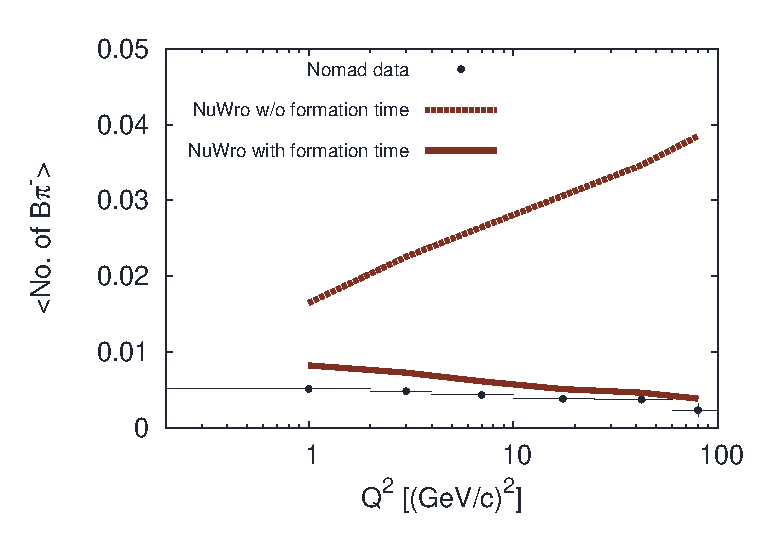
\includegraphics[width=0.5\slidewidth]{figures/nomad.eps}}
 
\end{slide}